\documentclass{article}
\makeindex

\usepackage{caption, amsmath, amsfonts, amssymb, amstext, amscd, amsthm, makeidx, graphicx, hyperref, url, inputenc, float, listings, color, titlesec, indentfirst}
\allowdisplaybreaks

\definecolor{dkgreen}{rgb}{0,0.6,0}
\definecolor{gray}{rgb}{0.5,0.5,0.5}
\definecolor{mauve}{rgb}{0.58,0,0.82}

\lstset{frame=tb,
  language=Java,
  aboveskip=3mm,
  belowskip=3mm,
  showstringspaces=false,
  columns=flexible,
  basicstyle={\small\ttfamily},
  numbers=none,
  numberstyle=\tiny\color{gray},
  keywordstyle=\color{blue},
  commentstyle=\color{dkgreen},
  stringstyle=\color{mauve},
  breaklines=true,
  breakatwhitespace=true,
  tabsize=3
}

\lstset{language=Python}

\pagenumbering{arabic}

\titleformat{\section}
  {\normalfont\Large\bfseries}{\thesection}{1em}{}

\topmargin -.5in
\textheight 9.0in

\title{Fine-tuning Segment Anything Model (SAM) for Satellite Detection in Aerial Images}
\author{Firdavs Nasriddinov}
\date{19 March 2024}

\begin{document}

\maketitle{}

\section*{Abstract}

In this report, we explore fine-tuning Meta's Segment Anything Model (SAM) for satellite detection in aerial images. SAM is a promptable segmentation system with zero-shot generalization to unfamiliar objects and images. To fine-tune SAM, we first load in a dataset of 1108 train images, 200 validation images and 200 test images where each image is a 512 x 641 grayscale image with a corresponding label that specifies the bounding box surrounding the satellite in view. We then segment each image with all SAM models of different sizes (base, large, huge) as well as MobileSAM (an optimized version of SAM developed for smaller-scale applications). We then iterate through each segmentation for each image and determine if any is within the bounding box for the satellite. With this, we can make a proper dataset for fine-tuning where we have a corresponding segmentation mask for the satellite in the image. This resulted in a final dataset of 411 training images, 102 validation images and 101 test images. In addition, we include another 25 test images without any satellites. Finally, for each image in the train and validation dataset, we resize the image to three difference sizes (512 x 512, 1024 x 1024, 2048 x 2048) and then get 256 x 256 patches of the resized images. We then discard all patches that don't contain any part of the satellite. We then train the SAM model for each resize size and test the model on the test set. We find that the 512 size model gets a test accuracy of 61.9\% with an average runtime of \_ seconds for each image. The 1024 size model gets a test accuracy of 54.0\% with an average runtime of \_ seconds for each image. The 2048 size model gets a test accuracy of \% with an average runtime of \_ seconds for each image. These runtimes are from running on a \_. Based on these results we conclude that the 512 size model is the best model for satellite detection in aerial images.

\medskip

\section*{Introduction}

\medskip

\section*{Methods and Results}

Each prepared image was gathered from United States Geological Survey (USGS) and satellites were artifically added into frame. The images were then segmented with different SAM checkpoints (base: 93.7 M parameters, large: 312 M parameters, huge: 641 M parameters) as well as MobileSAM (5 M parameters). Then, for each image, we iterate through each segmentation and determine if any is within the bounding box for the satellite. If so, we keep the segmentation mask correspoding to the satellite and discard the rest. 

\begin{figure}[H]
    \centering
    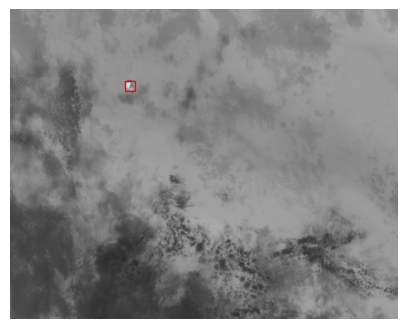
\includegraphics[width=0.4\textwidth]{figs/seg_img.png}\\
    $\Downarrow$\\
    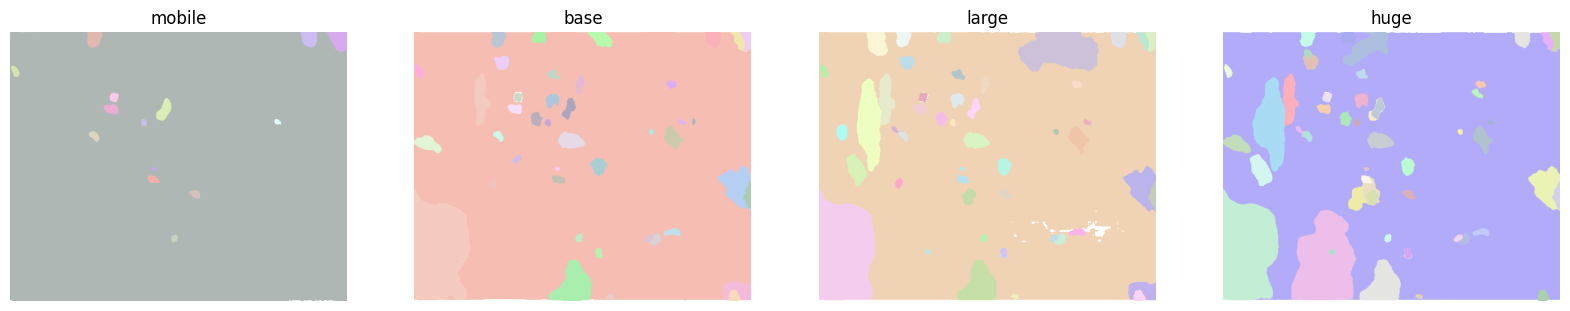
\includegraphics[width=1\textwidth]{figs/seg_overlays.png}\\
    $\Downarrow$\\
    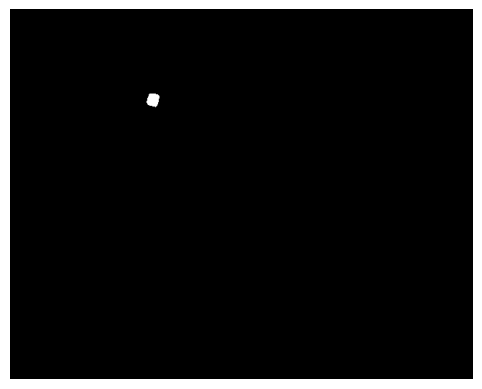
\includegraphics[width=0.4\textwidth]{figs/seg_mask.png}
    \captionsetup{width=.8\linewidth} 
    \caption{Example of generating satellite mask from input image. We first segment image through each SAM model and then determine segmentation mask within bounding box.}
\end{figure}

The final dataset for fine-tuning consisted of 411 training images, 102 validation images and 126 test images (25 without any satellites in view). Note that for training all images had satellites in view due to nature of fine-tuning SAM where there must be a valid non-empty segmentation mask for each image. 

For fine-tuning we load in the base SAM model from the transformers library and and only train the mask decoder layer. For each model size, we first train on the training set for 25 epochs with a learning rate of 0.00001 with Dice Cross-Enropy Loss (DiceCELoss) from the monai library. DiceCELoss returns the weighted average of the Dice loss [2] and cross-entropy loss between two input tensors. 

We make a prediction by first resizing the image to the corresponding image size that matches the model. We then split the image into 256 x 256 patches. We run the model on each patch. We then stitch the patches back together to get the final mask. Foe each patch, the model outputs logits for each pixel in the image. We apply a sigmoid to the logits to get probility matrix that has values between 0 and 1 for each pixel that corresponds to the likelihood of the pixel being a part of the satellite. We then threshold the probability matrix at a set value to get the final binary mask. We use the validation set to determine the best threshold value. We found that a threshold of 0.65 resulted in the highest validation accuracy. After, we resize the probabilty and prediction to the original image dimensions. Below is an example of a prediction.

\begin{figure}[H]
    \centering
    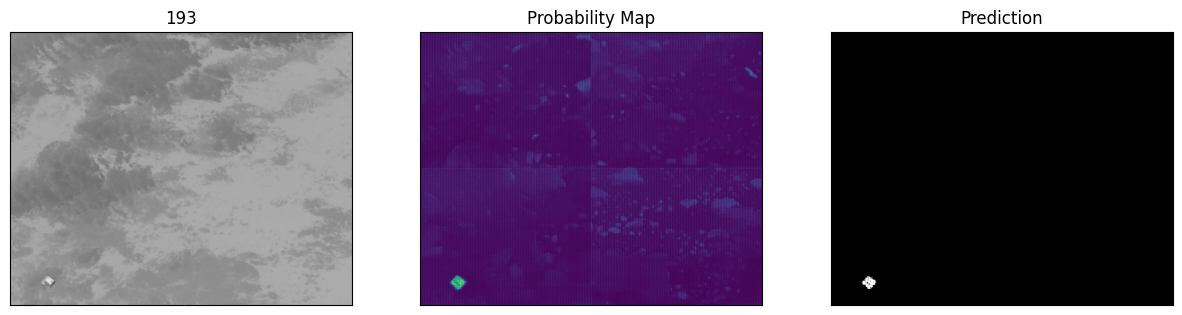
\includegraphics[width=1\textwidth]{figs/pred.png}\\
    \captionsetup{width=.8\linewidth} 
    \caption{Example of prediction for test image 193 with model size 512.}
\end{figure}

For determining the accuracy of the model, we use the joint intersection over union (IoU) metric. The joint IoU is the intersection over union of the predicted mask and the ground truth mask. We test that the joint intersection is over 50\% to mark it as a valid prediction. 

\medskip

\section*{Discussion}
\textit{1. Testing} \\

\begin{table}[H]
    \centering
    \begin{tabular}{ | c | c | c | }
        \hline
        Image/Model Size & Accuracy (\%) & Avg. Time (s) \\ 
        \hline
        512 & 61.9 & \\
        1024 & 54.0 & \\
        2047 & & \\
        \hline
    \end{tabular}
    \captionsetup{width=.8\linewidth} 
    \caption{Test accuracy and average runtime for each model size. Runtimes are from running on a Jetson TX2}
\end{table}

\textit{2. MSEPS Application}

\textit{3. Future Research}

\medskip

\section*{Conclusion}


\medskip

\begin{thebibliography}{9}

    \bibitem{kirillov2023}
        Alexander Kirillov, et al. 
        \textit{Segment anything}. 
        arXiv preprint arXiv:2304.02643, 2023.
    
    \bibitem{Sudre2017GeneralisedDO}
        Carole Helene Sudre, et al.
        \textit{Generalised Dice overlap as a deep learning loss function for highly unbalanced segmentations},
        Third International Workshop, DLMIA 2017, and 7th International Workshop, ML-CDS 2017, held in conjunction with MICCAI 2017 Quebec City, QC,...,
        2017, Vol. 2017, pp. 240--248.
        \url{https://api.semanticscholar.org/CorpusID:21957663}
    

\end{thebibliography}

\end{document}
